\documentclass[a4paper,12pt]{article}
\usepackage{lmodern}

\usepackage{multirow}
\usepackage{afterpage}
\usepackage{float}
\usepackage{ifthen}
\usepackage{framed}
\usepackage{xspace}
\usepackage{multicol}
\usepackage{enumitem}


\usepackage[dvips]{color}
\usepackage{titlesec}
\usepackage{gensymb}

\DeclareUnicodeCharacter{B0}{$\degree$}

%----------------------------------------
%dessin
\usepackage{amsmath,tikz}
\usepackage{verbatim}
\usetikzlibrary{shapes.geometric}
\usetikzlibrary{arrows}

%----------------------------------------
%couleur
\usepackage{colortbl}
\definecolor{darkred}{rgb}{.7,0.03,0.22}
\definecolor{red_tab}{rgb}{0.96,0.88,0.86}
\definecolor{darkblue}{HTML}{0000CC}
\definecolor{vdarkblue}{HTML}{000066}
\definecolor{texte}{HTML}{660099}
\definecolor{comt}{HTML}{009933}
%-----------------------------------------


%------------------------------------------
\newcounter{step}
\newcounter{substep}
\setcounter{step}{0}
\setcounter{substep}{0}
%------------------------------------------

\usepackage{tabularx}
\usepackage{makecell}


\newcolumntype{R}[1]{>{\raggedleft\arraybackslash }p{#1}}
\newcolumntype{L}[1]{>{\raggedright\arraybackslash }p{#1}}
\newcolumntype{C}[1]{>{\centering\arraybackslash }p{#1}}

\usepackage{wasysym}


\usepackage{ifluatex}
\ifluatex
\usepackage{fontspec}
\usepackage{polyglossia}
\setdefaultlanguage{slovak}
\else
\usepackage[utf8]{inputenc}
\usepackage[T1]{fontenc}
\usepackage[slovak]{babel}
\fi

%-----------------------------------------
%format page
\usepackage[a4paper,left=2cm,right=1cm,top=1cm,bottom=1cm,headheight=0cm, headsep=0cm, footskip=0cm,includefoot,includehead]{geometry}

%----------------------------------------
%numéro note de bas de page et entête
\usepackage{fancyhdr}
\pagestyle{fancy}
\renewcommand{\headrulewidth}{0pt}
\fancyhf{}

%-----------------------------------------
%lien hyper-texte
\usepackage[colorlinks, bookmarks, linkcolor=black, citecolor=black, urlcolor=blue]{hyperref}

%\setmainfont[Color=black]{Comic} %n'est pas géré par overleaf

\newcommand{\Style}[1]{
\ifthenelse{#1=1}{\makeatletter
\newcommand{\PrepTime}[1]{\def\@PrepTime{#1\xspace}
\def\PrepTimeb{#1}}
\newcommand{\CookingTime}[1]{\def\@CookingTime{#1\xspace}}
\newcommand{\CookingTempe}[1]{\def\@CookingTempe{#1}}
\newcommand{\TypeCooking}[1]{\def\@TypeCooking{#1}}
\newcommand{\NbPerson}[1]{\def\@NbPerson{#1\xspace}}
\newcommand{\Image}[2]{\def\@ImageDim{#1} \def\@ImagePath{#2}}
\def\maketitle{%

\clearpage
\newpage
\vspace{5cm} %?????
\begin{center}
{\Huge \@title}
\end{center}
}

\newenvironment{ingredient}
  {%\noindent\begingroup\edef\x{\endgroup\noexpand\includegraphics[width=1\linewidth,height=2.5cm,clip,viewport=\@ImageDim]{\@ImagePath}}\x
  \maketitle
  
  \begin{footnotesize}\noindent\begin{tabular}{|L{0.62\linewidth}|L{0.33\linewidth}|}\hline\vspace{-0.21cm}\underline{\textbf{{\normalsize Ingredients (\@NbPerson persons):}}} &\\
  \begin{minipage}{\linewidth}
  \vspace{0.2cm}
  }
  {\vspace{-0.2cm}
  \end{minipage}& \vspace{-1.8cm}Preparation time: \begin{tikzpicture}
  \pgfmathsetmacro{\timeor}{\PrepTimeb}
  \ifthenelse{\timeor>60}{
  \pgfmathsetmacro{\timeorb}{90-(\PrepTimeb-60)/60*360}
  \fill[orange] (0,0.55) arc(90:-270:0.55)      -- ++(-270:-0.55)
  arc(-270:0:0)    -- cycle;
  \fill[green] (0,0.55) arc(90:\timeorb:0.55)      -- ++(\timeorb:-0.55)
  arc(\timeorb:0:0)    -- cycle;
  }{
  \pgfmathsetmacro{\timeorb}{90-(\PrepTimeb)/60*360}
  \fill[orange] (0,0.55) arc(90:\timeorb:0.55)      -- ++(\timeorb:-0.55)
  arc(\timeorb:0:0)    -- cycle;
  }
  \node[fill=white,inner sep=0pt] at (0,0) {{\tiny \PrepTimeb~min}};
  \fill[black!50,even odd rule] (0,0) circle(0.65) circle(0.6);
  \fill[black!50,even odd rule] (0,0.5) circle(0.05);
  \fill[black!50,even odd rule] (0.5,0) circle(0.05);
  \fill[black!50,even odd rule] (0,-0.5) circle(0.05);
  \fill[black!50,even odd rule] (-0.5,0) circle(0.05);
  \end{tikzpicture} \par
  \vspace{0.2cm} Cooking: \@CookingTime min -- \@CookingTempe° \par \vspace{0.2cm} Type of cooking: \@TypeCooking \\\hline\end{tabular}\vspace{0.5cm} \end{footnotesize}}


\newenvironment{main}
  {\begin{multicols}{2}
  \begin{itemize}[label=$$]
  }
  {\end{itemize}\end{multicols}}
  
\newenvironment{subingredient}[1]
{\vspace{-0.3cm}\hspace{0.5cm}\underline{#1:}
\vspace{-0.3cm}\begin{multicols}{2}
\begin{itemize}[label=$$]
}
{\end{itemize}\end{multicols}}


\newenvironment{recipe}
{

}
{}
\makeatother

%-----------------------------------------
%nouveau environnements

\newenvironment{notes}
{\vfill\def\FrameCommand{\fboxsep=\FrameSep\fcolorbox{black}{white}}%
\MakeFramed {\advance\hsize-\width \FrameRestore}
\noindent\underline{\textbf{Notes and tips:}}%

\vspace{0.25cm}
\noindent\hspace{-0.15cm}}
{\vspace{2.5cm}\endMakeFramed}
  
  
\newcommand{\step}[1]{\ifthenelse{\value{step}=0}{\noindent{\large \underline{\textbf{Preparation:}}}\vspace{0.3cm}

}{}
\noindent\stepcounter{step}\setcounter{substep}{0}\the\value{step}. #1\vspace{0.3cm}

} 

\newcommand{\substep}[2][1]{\ifthenelse{\value{substep}=0}{\noindent\stepcounter{step}\the\value{step}. \underline{\textbf{#1:}}\vspace{0.3cm}

}{}
\hspace{0.3cm}\begin{minipage}{0.948\textwidth}
\noindent\stepcounter{substep}\roman{substep}. #2\vspace{0.5cm}
\end{minipage}

}   }{}
\ifthenelse{#1=2}{\makeatletter
\newcommand{\PrepTime}[1]{\def\@PrepTime{#1\xspace}
\def\PrepTimeb{#1}}
\newcommand{\CookingTime}[1]{\def\@CookingTime{#1\xspace}}
\newcommand{\CookingTempe}[1]{\def\@CookingTempe{#1}}
\newcommand{\TypeCooking}[1]{\def\@TypeCooking{#1}}
\newcommand{\NbPerson}[1]{\def\@NbPerson{#1\xspace}}
\newcommand{\Image}[2]{\def\@ImageDim{#1} \def \@ImagePath{#2}}
%\newcommand{\Style}[1]{\def\@Style{#1}}
\def\maketitle{

\vspace{0cm}
\begin{center}
{\Huge \@title}
\end{center}
}

\newenvironment{ingredient}
  {\noindent\begin{minipage}[t]{0.35\linewidth}
	
	%\includegraphics[height=5.5cm]{\@ImagePath}
	
  \def\FrameCommand{\fboxsep=\FrameSep\fcolorbox{black}{white}}%
  \MakeFramed {\advance\hsize-\width \FrameRestore}\begin{footnotesize}\noindent\underline{}}
  {\end{footnotesize}\endMakeFramed
    
    \end{minipage}\hspace{0.02\linewidth}}


\newenvironment{main}
  {\begin{itemize}[label=$$]
  }
  {\end{itemize}}
  
\newenvironment{subingredient}[1]
{\hspace{0.5cm}\underline{#1:}
\begin{itemize}[label=$$]
}
{\end{itemize}}

\newenvironment{recipe}
{\begin{minipage}[t]{0.62\linewidth}
%\vspace{-5cm}
%\maketitle
}
{\end{minipage}}
\makeatother


\newenvironment{notes}
{\vfill\def\FrameCommand{\fboxsep=\FrameSep\fcolorbox{black}{white}}%
\MakeFramed {\advance\hsize-\width \FrameRestore}
\noindent\underline{\textbf{Notes and tips:}}%

\vspace{0.25cm}
\noindent\hspace{-0.15cm}}
{\vspace{2.5cm}\endMakeFramed}
  

\newcommand{\step}[1]{\ifthenelse{\value{step}=0}{\noindent{\large \underline{\textbf{Preparation:}}}\vspace{0.3cm}

}{}
\noindent\stepcounter{step}\setcounter{substep}{0}\the\value{step}. #1\vspace{0.3cm}

} 

\newcommand{\substep}[2][1]{\ifthenelse{\value{substep}=0}{\noindent\stepcounter{step}\the\value{step}. \underline{\textbf{#1:}}\vspace{0.3cm}

}{}
\hspace{0.05\linewidth}\begin{minipage}{0.948\linewidth}
\noindent\stepcounter{substep}\roman{substep}. #2\vspace{0.5cm}
\end{minipage}

}   
}{}}
\Style{2}

\usepackage{hyperref}
\hypersetup{
    colorlinks=true,
    linkcolor=blue,
    filecolor=magenta,      
    urlcolor=blue,
}

\titleformat{\section}[block]{\Huge\bfseries\filcenter}{}{1em}{}
\titleformat{\subsection}[hang]{\Large\bfseries\filcenter}{}{1em}{}

\begin{document}
\renewcommand{\contentsname}{Obsah}
\tableofcontents
\newpage
\clearpage

%%%%%%% Jedna cast
\vspace*{10cm}
\section{Sladké jedlá}
\newpage
\clearpage

\setcounter{step}{0}
%------------------------------------------
% information doc
\subsection{Brownies}
\PrepTime{20}
\CookingTime{40}
\CookingTempe{175}
\TypeCooking{Pečenie}
\NbPerson{4}
\Image{0 0 430 430}{images/florentin} %style 2
%------------------------------------------

\begin{ingredient}
%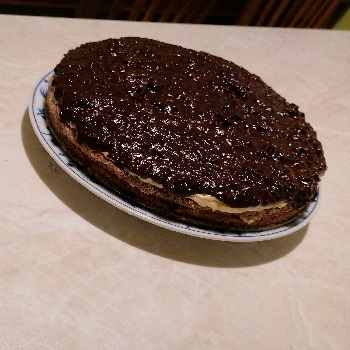
\includegraphics[height=5.5cm]{images/daim}
\def\portions{4}%
\textbf{{\normalsize Ingrediencie (\portions porcie):}}

\begin{main}
	\item 250g horká čokoláda
	\item 250g maslo
	\item 85g orechy
	\item 100g mliečna čokoláda na kúsky
	\item 100g biela čokoláda
	\item 175g hladká múka
	\item 1ČL prášok do pečiva
	\item 4 vajíčka
	\item 1 vanilkový cukor
	\item 300g kryštálový cukor
\end{main}
\end{ingredient}
\begin{recipe}
\textbf{{\normalsize Príprava:}}
\begin{enumerate}

\item{Čokoládu a maslo rozpustíme vo vodnom kúpeli}
\item{Pridáme múku a prášok do pečiva}
\item{Pridáme cukor, vajíčka, vanilkový cukor, orechy, pokrájanú čokoládu}	
\item{Pečieme 40 minút na 175°}

\end{enumerate}
\end{recipe}

\begin{notes}

\end{notes}
\clearpage	
\setcounter{step}{0}
%------------------------------------------
% information doc
\subsection{Cheesecake so slaným karamelom}
%------------------------------------------

\begin{ingredient}
%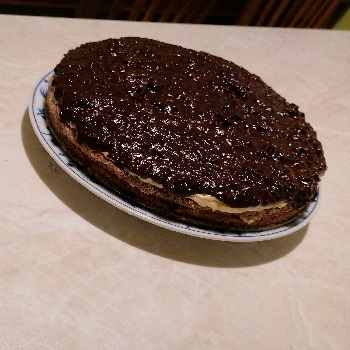
\includegraphics[height=5.5cm]{images/daim}
\def\portions{4}%
\textbf{{\normalsize Ingrediencie (\portions porcie):}}
%\vspace{0.5cm}
\begin{main}
	\item 
\end{main}
\begin{subingredient}{Cesto}
	\item 15g sušienky
	\item 80g maslo
\end{subingredient}
\begin{subingredient}{Plnka}
	\item 500g mascarpone
	\item 250g riccoty???/smotany??? salka???
	\item 3 vajíčka???
	\item 4PL cukor
\end{subingredient}
\begin{subingredient}{Slaný karamel}
	\item 150g kryštalóvý cukor
	\item 50g maslo
	\item 100ml smotana na šľahanie
	\item 0.5ČL soľ 	
\end{subingredient}

\end{ingredient}
\begin{recipe}
\textbf{{\normalsize Príprava:}}
\begin{enumerate}

\item{Maslové sušienky rozdrviť a primiešať maslo}
\item{Vystelieme formu na pečenie papierom a natlačíme na kraje sušienky s maslom}
\item{Dáme korpus piecť na 10-15 minút na 180° a zatiaľ zmiešame mascarpone s vajíčkami, cukrom, smotanou}	
\item{Zmesou naplníme korpus a dáme piecť na 40-50 minút}
\item{Pripravíme slaný karamel:}
\begin{enumerate}
\item{Skaramelizujeme cukor}
\item{Pridáme maslo}
\item{Prilejeme smotanu}
\item{Prídáme 1/2 lyžičky soli}
\end{enumerate}
\item{Polejeme, necháme v chladničke vychladnúť}

\end{enumerate}
\end{recipe}

\begin{notes}

\end{notes}
\clearpage	

\setcounter{step}{0}
%------------------------------------------
% information doc
\subsection{IKEA torta}
\PrepTime{45}
\CookingTime{35}
\CookingTempe{170}
\TypeCooking{Pečenie}
\NbPerson{4}
\Image{0 0 275 275}{images/daim} %style 2
%------------------------------------------

\begin{ingredient}
%\vspace{0.5cm}
\begin{main}
\item
\end{main}
\begin{subingredient}{Korpus}
	\item 4 bielka
	\item 150g kryštálový cukor
	\item 150g mandle + 30g vlašské orechy
\end{subingredient}
\begin{subingredient}{Plnka}
	\item 1 LIDL Piknik
	\item 40g múka
	\item 1 vanilkový cukor
	\item 75g maslo
	\item 4 žĺtka
\end{subingredient}
\begin{subingredient}{Posyp}
	\item DAIM čokoláda / krokant
	\item 125g čokoláda
	\item 50ml smotana/mlieko
\end{subingredient}
\begin{subingredient}{Krokant}
	\item 50g kryštálový cukor
	\item 20g orechy
	\item 1ČL maslo + 30ml voda
\end{subingredient}
\end{ingredient}%no space with \begin{recipe}
\begin{recipe}



\step{Pripravíme korpus}
\substep[Korpus]{bielka zmiešame s cukrom a vyšľaháme sneh}
\substep{pridáme orechy a len rukou domiešame aby sneh nespadol}
\substep{Dáme do vymúčenej formy a necháme piecť}

\step{Popri pečení pripravíme plnku:}

\substep[Plnka]{Žĺtka a salko miešame nad parou}
\substep{Pridáme cukor a múku}
\substep{Po vychladnutí primiešame maslo}

\step{Po upečení korpus rozrežeme a po vychladnutí naplníme plnkou}
\step{Na vrch dáme plnku a polejeme čokoládou zmiešanou s krokantom}


\end{recipe}

%\begin{notes}

%\end{notes}	
\setcounter{step}{0}
%------------------------------------------
% information doc
\subsection{Donuty}
\PrepTime{30}
\CookingTime{10}
\CookingTempe{180}
\TypeCooking{Vyprážanie}
\NbPerson{4}
\Image{0 0 275 275}{images/donuty} %style 2
%------------------------------------------

\begin{ingredient}
%\vspace{0.5cm}
\begin{main}
	\item štvrť maslo (65g)
	\item 2 PL kryštálový cukor
	\item vanilková aróma
	\item 1 vajce
	\item 2 hrnčeky polohrubá múka
\end{main}
\begin{subingredient}{Kvások}
	\item 1 hrnček teplé mlieko
	\item polovica droždie
	\item trošku cukor
\end{subingredient}
\end{ingredient}%no space with \begin{recipe}
\begin{recipe}



\step{Vyrobíme kvások a necháme 30 minút kysnúť}
\step{Zmiešame zvyšné ingrediencie s kváskom}
\step{Vyvaľkáme na 1,5cm a povykrajujeme donuty}	
\step{Rozohrejeme olej s ČL masla}
\step{Opražíme tak 10s z jednej a 10s z druhej strany}
\step{Podľa ľubovôle poleva z čokolády}

\end{recipe}

\begin{notes}

\end{notes}	
\setcounter{step}{0}
%------------------------------------------
% information doc
\subsection{Marshmallow fondán}
%------------------------------------------

\begin{ingredient}
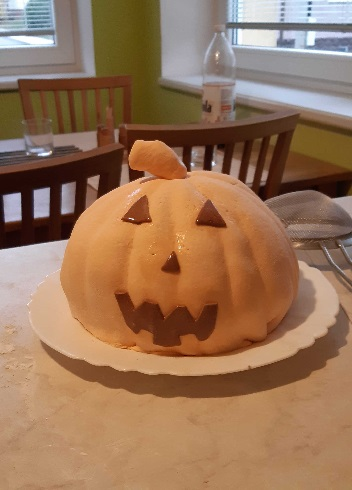
\includegraphics[height=5.5cm]{images/pistkot_krem_salko}
\def\portions{4}%
\textbf{{\normalsize Ingrediencie (\portions porcie):}}
%\vspace{0.5cm}
\begin{main}
	\item 200g marshmallow
	\item 1 ČL maslo
	\item 2 štipky kyseliny citrónovej
	\item 250g práškový cukor
\end{main}
\end{ingredient}
\begin{recipe}
\textbf{{\normalsize Príprava:}}
\begin{enumerate}

\item{Marshmallow, maslo a citrodeko dáme do misky a na minútu - dve do mikrovlnky. (Každých 15s premiešať.)}
\item{Pridávame preosiaty cukor. (Kým sa dá, miešame v miske)}
\item{Vyklopíme na dosku na preosiaty cukor, vyrobíme tuhšie cesto.}	
\item{Vyvaľkať a preniesť valčekom na tortu}

\end{enumerate}
\end{recipe}

\begin{notes}

\end{notes}
\clearpage	
\setcounter{step}{0}
%------------------------------------------
% information doc
\subsection{Fake kekse ku káve}
\PrepTime{15}
\CookingTime{10-15}
\CookingTempe{180}
\TypeCooking{Pečenie}
\NbPerson{4}
\Image{0 0 430 430}{images/florentin} %style 2
%------------------------------------------

\begin{ingredient}
%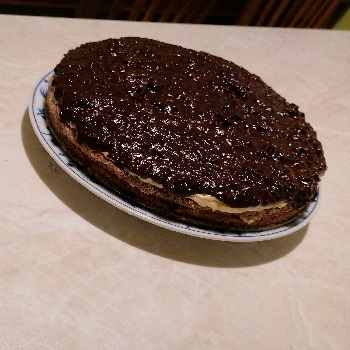
\includegraphics[height=5.5cm]{images/daim}
\def\portions{4}%
\textbf{{\normalsize Ingrediencie (\portions porcie):}}
%\vspace{0.5cm}
\begin{main}
	\item 125g maslo
	\item 125g cukor
	\item 2-3PL med
	\item 250g hladná múka
	\item štipka soli
	\item kypriaci prášok
\end{main}
\end{ingredient}
\begin{recipe}
\textbf{{\normalsize Príprava:}}
\begin{enumerate}


\item{Zmäknuté maslo vyšľahať s cukrom a štipkou soli}
\item{pridať múku s kypriacim práškom a med}
\item{Vyhnietiť do jemnej hmoty}	
\item{Nechať aspoň hodinu odpočinúť v chladničke}
\item{Vyvaľkať a vyťapkať z neho placky}
\item{Dať piecť do rúry}

\end{enumerate}
\end{recipe}

\begin{notes}

\end{notes}
\clearpage	
\setcounter{step}{0}
%------------------------------------------
% information doc
\subsection{Palacinky}
\PrepTime{10}
\CookingTime{5}
\CookingTempe{180}
\TypeCooking{Vyprážanie na sucho? dačo}
\NbPerson{1}
\Image{0 0 430 430}{images/palacinky} %style 2
%------------------------------------------

\begin{ingredient}
%\vspace{0.5cm}
\begin{main}
	\item 1 vajce
	\item 100g hladkej múky
	\item 100ml mlieko
	\item 1/4 vanilkového cukru, štipka soli
\end{main}
\end{ingredient}%no space with \begin{recipe}
\begin{recipe}



\step{Všetky zmiešame dokopy}
\step{Opekáme na panvici}

\end{recipe}

\begin{notes}

\end{notes}	
\setcounter{step}{0}
%------------------------------------------
% information doc
\subsection{Veterníky}
%------------------------------------------

\begin{ingredient}
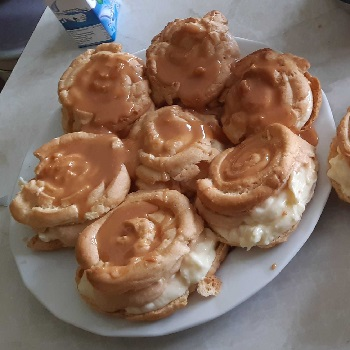
\includegraphics[height=5.5cm]{images/veterniky}
\def\portions{4}%
\textbf{{\normalsize Ingrediencie (\portions porcie):}}

\vspace{0.5cm}

\begin{subingredient}{Cesto}
	\item 300 ml voda
	\item 150g palmarín
	\item 150g hladká múka
	\item 4ks vajíčka
\end{subingredient}
\begin{subingredient}{Plnka 1}
	\item 1-2ks zlatý klas
	\item 750ml mlieko
	\item 1ks vanilkový cukor
	\item 3.5PL práškový cukor
	\item 125ml šľahačka
\end{subingredient}
\begin{subingredient}{Plnka 2}
	\item 10PL kryštálový cukor
	\item 500ml šľahačka
\end{subingredient}
\begin{subingredient}{Poleva}
	\item 2.5PL kryštálový cukor
	\item 25ml mlieko
	\item 125g práškový cukor
\end{subingredient}
\end{ingredient}
\begin{recipe}
\textbf{{\normalsize Príprava:}}
\begin{enumerate}

\item{Vodu s palmarínom necháme zovrieť a do toho pridáme múku.}
\item{Miešame 3 minúty nech sa cesto odliepa od hrnca. Necháme vychladnúť.}
\item{Do cesta primiešame vajíčka po jednom.}
\item{Na plech vytvarujeme ozdobným vreckom.}
\item{Pečieme 10 minút na 250C a potom 20 minút na 170C.}
\item{Ešte horúce veterníky rozrežeme.}

\item{Pripravíme karamel}
\begin{enumerate}
\item{Do hrnca dáme cukor aj na Plnku 2 aj na Polevu.}
\item{Časť karamelu pridáme do misky s cukrom na polevu, a zmiešame. (Ak je zmes hustá, pridáme \emph{kúsok} mlieka.)}
\item{Zvyšok karamelu si odložíme a neskôr pridáme k vymiešaným šľahačkám na Plnku 2.}
\end{enumerate}

\item{Urobíme puding na Plnku 1.}

\item{Pripravíme šľahačku}
\begin{enumerate}
\item{Vymiešame šľahačku na Plnku 1 aj na plnku 2}
\item{Po vychladnutí časť šľahačky primiešame do pudingu.}
\item{Do zvyšku primiešame karamel.}
\end{enumerate}

\item{Naplníme Plnkou 1, Plnkou 2 a polejeme Polevou}

\end{enumerate}
\end{recipe}

\begin{notes}

\end{notes}
\clearpage	
\setcounter{step}{0}
%------------------------------------------
% information doc
\subsection{Wafľe}
%------------------------------------------

\begin{ingredient}
%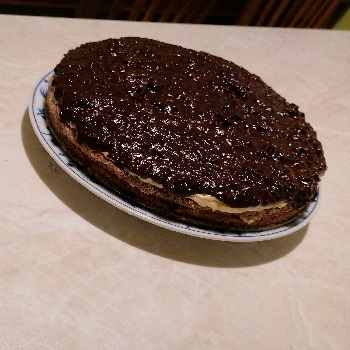
\includegraphics[height=5.5cm]{images/daim}
\def\portions{3}%
\textbf{{\normalsize Ingrediencie (\portions porcie):}}
%\vspace{0.5cm}
\begin{main}
	\item 150ml mlieko
	\item 3 vajce
	\item 7PL olej
	\item 175g hladká múka
	\item 1,5 PL cukor
	\item 1 prášok do pečiva
\end{main}
\end{ingredient}
\begin{recipe}
\textbf{{\normalsize Príprava:}}
\begin{enumerate}


\item{Všetko zmiešame dokopy}
\item{Vymastíme wafľovač, robíme wafle. (Ak sa trhajú, tak vajce/viac vymastiť)}

\end{enumerate}
\end{recipe}

\begin{notes}

\end{notes}
\clearpage	
\setcounter{step}{0}
%------------------------------------------
% information doc
\subsection{Pudingová torta}
\PrepTime{30}
\CookingTime{20}
\CookingTempe{180}
\TypeCooking{Pečenie}
\NbPerson{4}
\Image{0 0 430 430}{images/eh_torta} %style 2
%------------------------------------------

\begin{ingredient}
\vspace{0.3cm}

\begin{subingredient}{Piškótové cesto}
	\item 200g kryštálový cukor
	\item 1dl voda
	\item 4ks vajce
	\item 1dl olej (???)
	\item 200g hladká múka
	\item 1ks vanilkový cukor
	\item 1ks prášok do pečiva
\end{subingredient}
\begin{subingredient}{Pudingy}
	\item 500ml mlieka
	\item puding
	\item 2PL cukru
\end{subingredient}
\end{ingredient}%no space with \begin{recipe}
\begin{recipe}



\step{Urobíme piškótové cesto}
\substep[Piškótové cesto]{Žĺtka vymiešame s cukrami do peny}
\substep{Pridáme olej a vodu a premiešame}
\substep{Pridáme múku s práškom do pečiva}
\substep{Pridáme sneh z bielok}
\substep{Pečieme 20 minút na 180°C}

\step{Urobíme puding a vykydneme na piškót}	
\step{Pred podávaním necháme vychladiť v chladničke}

\end{recipe}

\begin{notes}

\end{notes}	
\setcounter{step}{0}
%------------------------------------------
% information doc
\subsection{TODO}
\PrepTime{45}
\CookingTime{10}
\CookingTempe{180}
\TypeCooking{Plaque}
\NbPerson{4}
\Image{0 0 430 430}{images/florentin} %style 2
%------------------------------------------

\begin{ingredient}
%\vspace{0.5cm}
\begin{main}
	\item 4 cà.S de sucre en poudre
	\item 1 cà.S de crème liquide
	\item 1 cà.S de miel
	\item 1 grosse noix de beurre
	\item 35 gr d’amandes effilées
	\item 50 gr de chocolat au lait ou chocolat blanc
\end{main}
\begin{subingredient}{Test subingredient}
	\item 1 cà.c de test1
	\item 1 à 2 cà.S de test2
	\item 3 gouttes de test3
	\item 8 morceaux de test4.	
\end{subingredient}
\end{ingredient}%no space with \begin{recipe}
\begin{recipe}


\textbf{Nájsť recept}
\step{Préchauffez votre four à 180°C (th.6).}
\step{Dans une casserole, faites bouillir le sucre en poudre avec la crème liquide, le beurre et le miel.}
\step{Une fois que le sucre prend une jolie coloration brune, versez les amandes effilées dans la casserole, et remuez bien pour napper l’intégralité des amandes.}	
\step{Pour la cuisson au four vous avez 2 possibilités : Soit vous versez la « pâte » dans le fond de moules en silicone, type moules à muffins ou moules à tartelettes, soit vous étalez bien la « pâte », et rapidement car le caramel durcit vite, sur la plaque de votre four recouverte d’une feuille de papier sulfurisé, et après la cuisson vous découperez des cercles à l’aide d’un emporte-pièces rond.}
\step{Dans tous les cas, mettez la « pâte » au four pendant 3 à 5 minutes. A la sortie du four, soit vous découpez tout de suite des ronds à l’aide de l’emporte-pièces, soit vous laissez refroidir les florentins avant de les démouler de vos moules à muffins.}
\step{Pendant que les florentins refroidissent, faites fondre le chocolat au lait ou blanc soit au bain-marie, soit au micro-ondes à faible puissance, soit dans une petite casserole à feu doux.}
\step{Trempez ensuite la moitié des florentins dans le chocolat fondu et mettez-les au réfrigérateur pendant une bonne vingtaine de minutes pour que le chocolat prenne bien.}
\substep[Test substep]{Blabla}
\substep{Blabla}

\end{recipe}

\begin{notes}

\end{notes}	
\setcounter{step}{0}
%------------------------------------------
% information doc
\subsection{Piškótové cesto}
%------------------------------------------

\begin{ingredient}
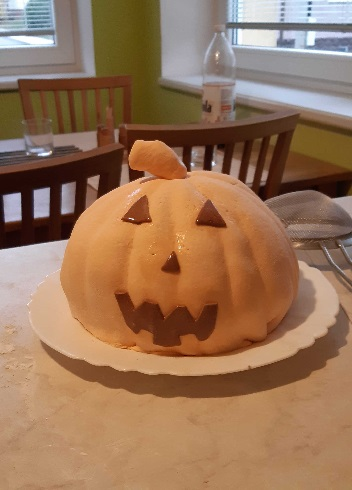
\includegraphics[height=5.5cm]{images/pistkot_krem_salko}
\def\portions{8}%
\textbf{{\normalsize Ingrediencie (\portions porcie):}}
%\vspace{0.5cm}
\begin{main}
	\item 6 vajíčko
	\item 6 lyžíc polohrubá múka
	\item 6 lyžíc cukor
\end{main}
\end{ingredient}
\begin{recipe}
\textbf{{\normalsize Príprava:}}
\begin{enumerate}
\item{Vajíčka vyšľaháme do peny}
\item{Po lyžiciach pridávame cukor a potom múku}
\item{Pečieme 20-25 minút na 180°}
\end{enumerate}
\end{recipe}

\begin{notes}

\end{notes}
\clearpage	
\setcounter{step}{0}
%------------------------------------------
% information doc
\subsection{Salko krém na tortu}
\PrepTime{10}
\CookingTime{0}
\CookingTempe{0}
\TypeCooking{Mixovanie}
\NbPerson{4}
\Image{0 0 400 400}{images/pistkot_krem_salko} %style 2
%------------------------------------------

\begin{ingredient}
%\vspace{0.5cm}
\begin{main}
	\item 250g maslo
	\item 1 konzerva uvareného salka
\end{main}
\end{ingredient}%no space with \begin{recipe}
\begin{recipe}



\step{Maslo vyložíme z chladničky a necháme zmäknúť.}
\step{Maslo mixujeme a popri tom po lyžiciach pridávame salko}


\end{recipe}

\begin{notes}

\end{notes}	
\setcounter{step}{0}
%------------------------------------------
% information doc
\subsection{Listkove cesto}
%------------------------------------------

\begin{ingredient}
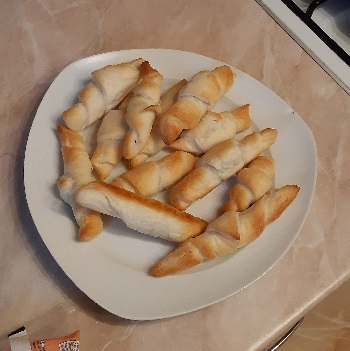
\includegraphics[height=5.5cm]{images/listkove_cesto}
\def\portions{4}%
\textbf{{\normalsize Ingrediencie (\portions porcie):}}
%\vspace{0.5cm}
\begin{main}
	\item chladené lístkové cesto
\end{main}
\begin{subingredient}{Inšpirácia na plnku}
	\item nuttela
	\item paradajkový pretlak, šunka, syr, pizza korenie
	\item puding
	\item jablko
	\item mak
	\item tvaroh
\end{subingredient}
\end{ingredient}
\begin{recipe}
\textbf{{\normalsize Príprava:}}
\begin{enumerate}
\item{Cesto necháme chvíľočku ohriať}
\item{Robíme croisanty, pizzové rolky, pudingové taštičky, jablkové taštičky, mak, jablko, tvaroh, hocičo}
\item{Pečieme zhruba 15 minút na 200}
\end{enumerate}
\end{recipe}

\begin{notes}

\end{notes}
\clearpage	


%%%%%%% Jedna cast
\vspace*{10cm}
\section{Slané jedlá}
\newpage
\clearpage

\setcounter{step}{0}
%------------------------------------------
% information doc
\subsection{Džadky}
\PrepTime{45}
\CookingTime{10}
\CookingTempe{180}
\TypeCooking{Varenie+praženie}
\NbPerson{4}
\Image{0 0 430 430}{images/florentin} %style 2
%------------------------------------------

\begin{ingredient}
%\vspace{0.5cm}
\begin{main}
	\item 1kg zemiaky
	\item 100g múka (asi hrubá)
	\item 2KL soľ
	\item slanina
	
\end{main}
\end{ingredient}%no space with \begin{recipe}
\begin{recipe}

\step{Očistiť zemiaky, dať variť aby boli tesne zakryté vodou}
\step{Zamiaky popučiť vo vode}
\step{Pridať múku}	
\step{Nechať postáť, aby múka v horúcich zemiakoch napučala}
\step{Vyvaľkať džadky}
\step{Popražiť na panvici}
\step{Posypať opraženou slaninkou}

\end{recipe}

\begin{notes}

\end{notes}	
\setcounter{step}{0}
%------------------------------------------
% information doc
\subsection{Lokše}
\PrepTime{10}
\CookingTime{10}
\CookingTempe{180}
\TypeCooking{Opečenie}
\NbPerson{4}
\Image{0 0 430 430}{images/florentin} %style 2
%------------------------------------------

\begin{ingredient}
%\vspace{0.5cm}
\begin{main}
	\item Zemiaky čo zostali z obeda
	\item Trocha múky
	\item olivový olej
	\item cesnak
\end{main}
\end{ingredient}%no space with \begin{recipe}
\begin{recipe}



\step{Zmiešame zemiaky čo zostali z obeda s trochou múky}
\step{Rozvaľkáme/v rukách roztlačíme}
\step{Pomúčené opekáme, aby sa nepripaľovalo}	
\step{Zmiešať pretlačený cesnak s olivovým olejom}

\end{recipe}

\begin{notes}

\end{notes}	
\setcounter{step}{0}
%------------------------------------------
% information doc
\subsection{Obrátené rezne}
\PrepTime{45}
\CookingTime{30-40}
\CookingTempe{180}
\TypeCooking{Pečnie/praženie}
\NbPerson{4}
\Image{0 0 430 430}{images/florentin} %style 2
%------------------------------------------

\begin{ingredient}
%\vspace{0.5cm}
\begin{main}
	\item bravčové mäso
	\item olej
	\item soľ
	\item čierne korenie
	\item strúhanka
	\item vajcia
	\item cibuľa
\end{main}
\begin{subingredient}{Nálev}
	\item maslo
	\item olej
	\item soľ
	\item vegeta
	\item kečup
	\item horčica
	\item čierne korenie
\end{subingredient}
\end{ingredient}%no space with \begin{recipe}
\begin{recipe}

\step{Mäso naklepeme a nakoreníme}
\step{Do mäsa vkepeme strúhanku}
\step{Namočíme vo vajíčku a sprudka opražíme}	
\step{Vymastiť plech}
\step{Pokrájať cibuľu na kolieska a poukladať na rezne na plech}
\substep[Nálev]{Rozpustiť maslo s olejom}
\substep{Pridať soľ, vegetu, kečup, horčicu, korenie}
\substep{Prevariť na sporáku}
\step{Vyliať na rezne}
\step{Zakryť alobalom a dať piecť}
\step{5 minút na najsilnejšom}
\step{20-30 minút na 180°C}
\step{5 minút bez alobalu}

\end{recipe}

\begin{notes}

\end{notes}	
\setcounter{step}{0}
%------------------------------------------
% information doc
\subsection{Florentins au chocolat}
\PrepTime{45}
\CookingTime{10}
\CookingTempe{180}
\TypeCooking{Plaque}
\NbPerson{4}
\Image{0 0 430 430}{images/florentin} %style 2
%------------------------------------------

\begin{ingredient}
%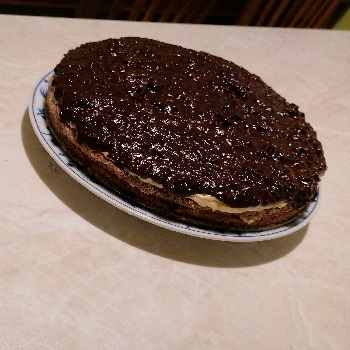
\includegraphics[height=5.5cm]{images/daim}
\def\portions{4}%
\textbf{{\normalsize Ingrediencie (\portions porcie):}}
%\vspace{0.5cm}
\begin{main}
	\item 4 cà.S de sucre en poudre
	\item 1 cà.S de crème liquide
	\item 1 cà.S de miel
	\item 1 grosse noix de beurre
	\item 35 gr d’amandes effilées
	\item 50 gr de chocolat au lait ou chocolat blanc
\end{main}
\begin{subingredient}{Test subingredient}
	\item 1 cà.c de test1
	\item 1 à 2 cà.S de test2
	\item 3 gouttes de test3
	\item 8 morceaux de test4.	
\end{subingredient}
\end{ingredient}
\begin{recipe}
\textbf{{\normalsize Príprava:}}
\begin{enumerate}


\item{Préchauffez votre four à 180°C (th.6).}
\item{Dans une casserole, faites bouillir le sucre en poudre avec la crème liquide, le beurre et le miel.}
\item{Une fois que le sucre prend une jolie coloration brune, versez les amandes effilées dans la casserole, et remuez bien pour napper l’intégralité des amandes.}	
\item{Pour la cuisson au four vous avez 2 possibilités : Soit vous versez la « pâte » dans le fond de moules en silicone, type moules à muffins ou moules à tartelettes, soit vous étalez bien la « pâte », et rapidement car le caramel durcit vite, sur la plaque de votre four recouverte d’une feuille de papier sulfurisé, et après la cuisson vous découperez des cercles à l’aide d’un emporte-pièces rond.}
\item{Dans tous les cas, mettez la « pâte » au four pendant 3 à 5 minutes. A la sortie du four, soit vous découpez tout de suite des ronds à l’aide de l’emporte-pièces, soit vous laissez refroidir les florentins avant de les démouler de vos moules à muffins.}
\item{Pendant que les florentins refroidissent, faites fondre le chocolat au lait ou blanc soit au bain-marie, soit au micro-ondes à faible puissance, soit dans une petite casserole à feu doux.}
\item{Trempez ensuite la moitié des florentins dans le chocolat fondu et mettez-les au réfrigérateur pendant une bonne vingtaine de minutes pour que le chocolat prenne bien.}

\end{enumerate}
\end{recipe}

\begin{notes}

\end{notes}
\clearpage	
\setcounter{step}{0}
%------------------------------------------
% information doc
\subsection{Pizza}
%------------------------------------------

\begin{ingredient}
%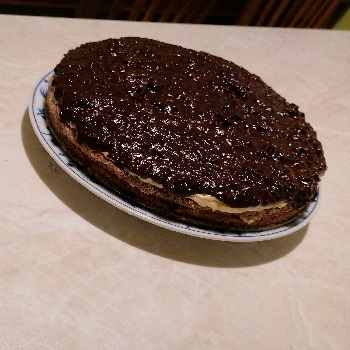
\includegraphics[height=5.5cm]{images/daim}
\def\portions{4}%
\textbf{{\normalsize Ingrediencie (\portions porcie):}}
%\vspace{0.5cm}
\begin{main}
	\item šunka
	\item syr
	\item paradajkový pretlak
	\item pizza korenie, oregáno
	\item cibuľa
	\item vajíčko (potom ale pečieme pomalšie)
\end{main}
\begin{subingredient}{Cesto}
	\item 1 cà.c de test1
	\item 1 à 2 cà.S de test2
	\item 3 gouttes de test3
	\item 8 morceaux de test4.	
\end{subingredient}

\begin{subingredient}{Syrová omáčka}
	\item niva/rival
	\item syr v črievku
	\item smotana na varenie/na šľahanie
	\item nastrúhaný syr
\end{subingredient}
\end{ingredient}
\begin{recipe}
\textbf{{\normalsize Príprava:}}
\begin{enumerate}

\item{Urobíme cesto:}
\begin{enumerate}
\item{Blabla}
\item{Blabla}
\item{Blabla}
\item{Blabla}
\end{enumerate}
\item{Na cesto dáme veci, podľa chuti}

\item{Syrová pizza:}
\begin{enumerate}
\item{Postrúhame tvrdý syr}
\item{zmiešame so smotanou, plesnivým syrom, syrom v črievku}
\item{Natrieme na pizzu}
\end{enumerate}

\end{enumerate}
\end{recipe}

\begin{notes}

\end{notes}
\clearpage	
\setcounter{step}{0}
%------------------------------------------
% information doc
\subsection{Lasagne s brokolicou}
\PrepTime{45}
\CookingTime{30}
\CookingTempe{180}
\TypeCooking{Pečenie}
\NbPerson{4}
\Image{0 0 430 430}{images/florentin} %style 2
%------------------------------------------

\begin{ingredient}
%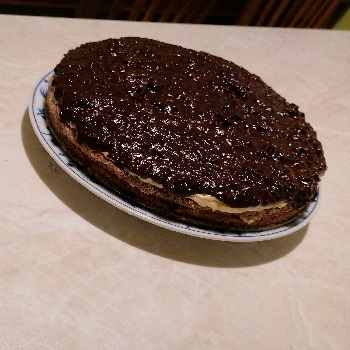
\includegraphics[height=5.5cm]{images/daim}
\def\portions{4}%
\textbf{{\normalsize Ingrediencie (\portions porcie):}}
%\vspace{0.5cm}
\begin{main}
	\item lasagnové pláty
	\item brokolica
	\item tvrdý syr
\end{main}
\begin{subingredient}{Bešamel}
	\item 50g maslo
	\item štipka soli
	\item 100g hladkej múky
	\item 500ml mlieka
	\item nejaké korenie
\end{subingredient}
\end{ingredient}
\begin{recipe}
\textbf{{\normalsize Príprava:}}
\begin{enumerate}

\item{Uvaríme brokolicu}
\item{Pripravíme si bešamel:}
\begin{enumerate}
\item{Roztopiť maslo, pridať múku}
\item{Pridávať mlieko}
\item{Osoliť, okoreniť}
\end{enumerate}

\item{Dáme do taniera vriacu vodu, postupne do nej namáčame pláty a ukladáme do zapekacej misy}
\item{Na vrstvu plátov dáme vrstvu bešamelu a brokolice (poprípade šunky)}
\item{Na poslednú vrstvu nedávame brokolicu, ale poukladáme/postrúhame tvrdý syr}

\end{enumerate}
\end{recipe}

\begin{notes}

\end{notes}
\clearpage	
\setcounter{step}{0}
%------------------------------------------
% information doc
\subsection{Cestoviny}
\PrepTime{15}
\CookingTime{10}
\CookingTempe{180}
\TypeCooking{Varenie}
\NbPerson{4}
\Image{0 0 430 430}{images/cestoviny} %style 2
%------------------------------------------

\begin{ingredient}
%\vspace{0.5cm}
\begin{main}
	\item cestoviny, 100g na človeka
\end{main}
\begin{subingredient}{Omáčka}
	\item rival/niva
	\item karička/bambino
	\item smotana
	\item olivy
	\item sušené paradajky 
	\item špenát 
	\item kuracie mäso
	\item cibuľka 
	\item cesnak
\end{subingredient}
\end{ingredient}%no space with \begin{recipe}
\begin{recipe}

\step{Uvaríme cestoviny}
\step{Na cibuľke popražíme paradajky a mäso}
\step{Zalejeme smotanou, pridáme syry, špenát, olivy}	

\end{recipe}

\begin{notes}

\end{notes}	
\setcounter{step}{0}
%------------------------------------------
% information doc
\subsection{Mäso s bylinkovým maslom}
%------------------------------------------

\begin{ingredient}
%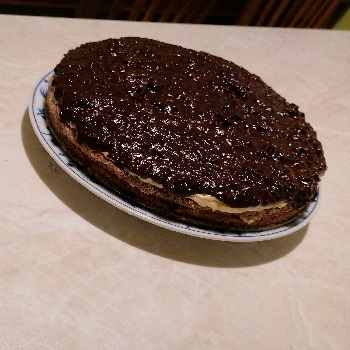
\includegraphics[height=5.5cm]{images/daim}
\def\portions{4}%
\textbf{{\normalsize Ingrediencie (\portions porcie):}}
%\vspace{0.5cm}
\begin{main}
	\item kuracie mäso
	\item PL maslo
	\item šunka
	\item cesnak
	\item pažitka
	\item trojobal
\end{main}
\end{ingredient}
\begin{recipe}
\textbf{{\normalsize Príprava:}}
\begin{enumerate}

\item{Maslo zmiešať s cesnakom a bylinkami urobiť guľku, a dať do mrazničky}
\item{Spraviť otvor do mäsa, kde vložíme v šunke zabalené maslo}
\item{Obaliť v trojobale}	
\item{Vypražiť}

\end{enumerate}
\end{recipe}

\begin{notes}

\end{notes}
\clearpage	
\setcounter{step}{0}
%------------------------------------------
% information doc
\subsection{UBO k mäsu}
\PrepTime{10}
\CookingTime{10}
\CookingTempe{180}
\TypeCooking{Varenie}
\NbPerson{4}
\Image{0 0 430 430}{images/florentin} %style 2
%------------------------------------------

\begin{ingredient}
%\vspace{0.5cm}
\begin{main}
	\item rival/niva
	\item karička/bambino
	\item smotana
	\item vegeta
	\item cibuľa
\end{main}
\end{ingredient}%no space with \begin{recipe}
\begin{recipe}

\step{Rovnako ako omáčka na cestoviny popražiť cibuľku}
\step{Pridať smotanu, syry, soľ, vegetu}

\end{recipe}

\begin{notes}

\end{notes}	
\setcounter{step}{0}
%------------------------------------------
% information doc
\subsection{Tapenarde}
%------------------------------------------

\begin{ingredient}
%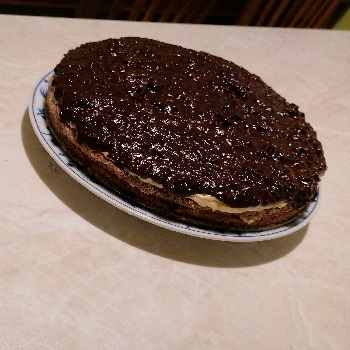
\includegraphics[height=5.5cm]{images/daim}
\def\portions{4}%
\textbf{{\normalsize Ingrediencie (\portions porcie):}}
%\vspace{0.5cm}
\begin{main}
	\item 100 g olivy 
	\item 5ks kapari
	\item štipka čierne korenie
	\item štipka soľ
	\item 2PL olivový olej
	\item 1ČL štava z citrónu
	\item štipka tymián
\end{main}
\end{ingredient}
\begin{recipe}
\textbf{{\normalsize Príprava:}}
\begin{enumerate}


\item{Všetko zmiešame dokopy}
\item{Pomixujeme ponorným mixérom}

\end{enumerate}
\end{recipe}

\begin{notes}

\end{notes}
\clearpage	

\setcounter{step}{0}
%------------------------------------------
% information doc
\subsection{Varená kukurica}
%------------------------------------------

\begin{ingredient}
%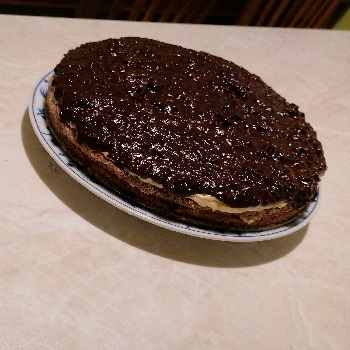
\includegraphics[height=5.5cm]{images/daim}
\def\portions{4}%
\textbf{{\normalsize Ingrediencie (\portions porcie):}}
%\vspace{0.5cm}
\begin{main}
	\item kukurica
	\item soľ
	\item maslo
\end{main}
\end{ingredient}
\begin{recipe}
\textbf{{\normalsize Príprava:}}
\begin{enumerate}

\item{Dáme variť vodu s kukuricou, môžeme do vody pridať zopár šupiek z kukurice}
\item{Varíme 5 minút}

\end{enumerate}
\end{recipe}

\begin{notes}

\end{notes}
\clearpage	


%%%%%%% Jedna cast
\vspace*{10cm}
\section{Polievky}
\newpage
\clearpage

\setcounter{step}{0}
%------------------------------------------
% information doc
\subsection{Basic polievka}
\PrepTime{10}
\CookingTime{10}
\CookingTempe{180}
\TypeCooking{Varenie}
\NbPerson{2}
\Image{0 0 430 430}{images/florentin} %style 2
%------------------------------------------

\begin{ingredient}
%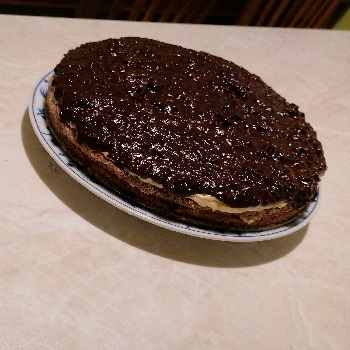
\includegraphics[height=5.5cm]{images/daim}
\def\portions{2}%
\textbf{{\normalsize Ingrediencie (\portions porcie):}}
%\vspace{0.5cm}
\begin{main}
	\item PL múka
	\item 2PL múka
	\item cibuľa/párky/zemiaky/cesnak
	\item vegeta
	\item soľ
	\item voda
\end{main}
\end{ingredient}
\begin{recipe}
\textbf{{\normalsize Príprava:}}
\begin{enumerate}

\item{Urobíme zápraž/šku}
\begin{enumerate}
\item{Zohriať olej}
\item{Popražiť cibuľa/párky/cesnak}
\item{Pridať múku}
\end{enumerate}
\item{Pridať vodu, soľ, vegetu, zemiaky/(paradajkový pretlak, cibuľu, bobkový list, cukor)}
\item{Pridať oregáno/majoránku/cesnak}


\end{enumerate}
\end{recipe}

\begin{notes}

\end{notes}
\clearpage	
\setcounter{step}{0}
%------------------------------------------
% information doc
\subsection{Kapustnica}
\PrepTime{45}
\CookingTime{60}
\CookingTempe{180}
\TypeCooking{Varenie}
\NbPerson{4}
\Image{0 0 430 430}{images/kapustnica} %style 2
%------------------------------------------

\begin{ingredient}
%\vspace{0.5cm}
\begin{main}
	\item zemiaky
	\item klobása
	\item kyslá kapusta
	\item sušené hríby
	\item červená paprika
	\item zápraš/žka
\end{main}
\end{ingredient}%no space with \begin{recipe}
\begin{recipe}

\step{Pokrajáné zemiaky variť s polovicou klobás, hubami a okoreniť, osoliť}
\step{Pridať kapustu}
\step{Urobíme zápraš/žku s klobásou a paprikou}
\step{Zmiešame dokopy, a prevrieme}

\end{recipe}

\begin{notes}

\end{notes}	

\setcounter{step}{0}
%------------------------------------------
% information doc
\subsection{Hrášková krémová}
\PrepTime{15}
\CookingTime{10}
\CookingTempe{180}
\TypeCooking{Varenie}
\NbPerson{4}
\Image{0 0 430 430}{images/florentin} %style 2
%------------------------------------------

\begin{ingredient}
%\vspace{0.5cm}
\begin{main}
	\item konzerva hrášku
	\item smotana
	\item zemiak??
\end{main}
\end{ingredient}%no space with \begin{recipe}
\begin{recipe}

\step{Konzervu zliať z trochu vody, pridať smotanu a rozmixovať}
\step{Osoliť, ovegetiť, dať variť.}
\step{Čo ten zemiak?}	

\end{recipe}

\begin{notes}

\end{notes}	
\setcounter{step}{0}
%------------------------------------------
% information doc
\subsection{Fazuľová polievka}
%------------------------------------------

\begin{ingredient}
%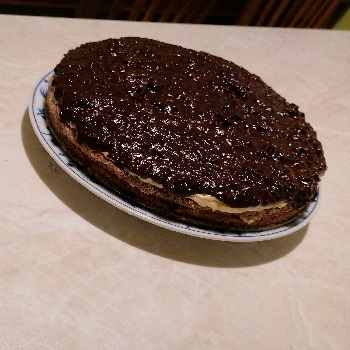
\includegraphics[height=5.5cm]{images/daim}
\def\portions{4}%
\textbf{{\normalsize Ingrediencie (\portions porcie):}}
%\vspace{0.5cm}
\begin{main}
	\item 150g fazuľa
	\item cibuľa
	\item bobkový list
	\item zemiaky
	\item smotana
	\item klobása
	\item červená paprika
	\item hladká múka
\end{main}
\end{ingredient}
\begin{recipe}
\textbf{{\normalsize Príprava:}}
\begin{enumerate}

\item{Deň vopred si fazuľu namočíme do vody (koľko vypije, toľko)}
\item{Uvaríme fazuľu s klobásou, bobkovým listom a cibuľou, osolíme}
\item{Keď je fazuľa skoro mäkká pridáme zemiaky}
\item{V smotane rozmiešame hladkú múku a červenú papriku}
\item{Zmiešame a necháme prevrieť}	

\end{enumerate}
\end{recipe}

\begin{notes}

\end{notes}
\clearpage	
\setcounter{step}{0}
%------------------------------------------
% information doc
\subsection{Brokolicová polievka}
%------------------------------------------

\begin{ingredient}
%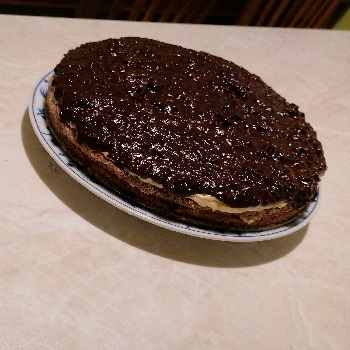
\includegraphics[height=5.5cm]{images/daim}
\def\portions{4}%
\textbf{{\normalsize Ingrediencie (\portions porcie):}}
%\vspace{0.5cm}
\begin{main}
	\item Brokolica
	\item 1 smotana na šľahanie
	\item soľ
    \item vegeta
    \item zemiaky
	
\end{main}

\end{ingredient}
\begin{recipe}
\textbf{{\normalsize Príprava:}}
\begin{enumerate}

\item{Brokolicu so zemiakmi posolíme a dáme variť}
\item{Po zmäknutí zalejeme smotanou na šľahanie a pomixujeme}
\item{Ovegetíme, necháme prevrieť}	

\end{enumerate}
\end{recipe}

\begin{notes}

\end{notes}
\clearpage	

\setcounter{step}{0}
%------------------------------------------
% information doc
\subsection{Hubová krémová}
\PrepTime{15}
\CookingTime{10}
\CookingTempe{180}
\TypeCooking{Varenie}
\NbPerson{4}
\Image{0 0 430 430}{images/florentin} %style 2
%------------------------------------------

\begin{ingredient}
%\vspace{0.5cm}
\begin{main}
	\item rozumne huby
	\item 250ml smotana na varenie
	\item soľ, vegeta
	\item zemiaky
	\item cibuľa
\end{main}
\end{ingredient}%no space with \begin{recipe}
\begin{recipe}



\step{Popražíme cibuľu a pridáme huby}
\step{Zalejeme vodou, pridáme zemiaky, dochutíme, necháme prevrieť}
\step{Pridáme smotanu, pomixujeme}
\step{Necháme prevrieť}

\end{recipe}

\begin{notes}

\end{notes}	
\setcounter{step}{0}
%------------------------------------------
% information doc
\subsection{Hokaido krémová}
\PrepTime{15}
\CookingTime{10}
\CookingTempe{180}
\TypeCooking{Varenie}
\NbPerson{4}
\Image{0 0 430 430}{images/florentin} %style 2
%------------------------------------------

\begin{ingredient}
%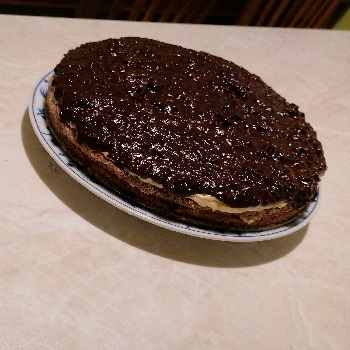
\includegraphics[height=5.5cm]{images/daim}
\def\portions{4}%
\textbf{{\normalsize Ingrediencie (\portions porcie):}}
%\vspace{0.5cm}
\begin{main}
	\item 1 tekvica hokaido
	\item 250ml smotana na varenie
	\item soľ, vegeta
	\item cibuľa
\end{main}
\end{ingredient}
\begin{recipe}
\textbf{{\normalsize Príprava:}}
\begin{enumerate}



\item{Popražíme cibuľu a pridáme umytú nakrájanú tekvicu (aj so šupkou)}
\item{Zalejeme vodou, dochutíme, necháme prevrieť}
\item{Pridáme smotanu, pomixujeme}
\item{Necháme prevrieť}

\end{enumerate}
\end{recipe}

\begin{notes}

\end{notes}	
\clearpage
\setcounter{step}{0}
%------------------------------------------
% information doc
\subsection{Paradajková polievka}
\PrepTime{15}
\CookingTime{10}
\CookingTempe{180}
\TypeCooking{Varenie}
\NbPerson{4}
\Image{0 0 430 430}{images/florentin} %style 2
%------------------------------------------

\begin{ingredient}
%\vspace{0.5cm}
\begin{main}
	\item 500ml pasírované paradajky / 250g pretlak
	\item 1 bobkový list
	\item 2PL cukor
	\item 1ČL soľ
	\item strúhaný tvrdý syr
	\item olej, hladká múka
	\item vegeta
	\item cibuľa
\end{main}
\end{ingredient}%no space with \begin{recipe}
\begin{recipe}

\step{Urobíme zápraš/žku}
\step{Zalejeme vodou, pridáme paradajky, osolíme, ovegetíme, pridáme bobkový list}
\step{Necháme prevrieť}

\end{recipe}

\begin{notes}

\end{notes}	


%%%%%%% Jedna cast
\vspace*{10cm}
\section{Template}
\newpage
\clearpage

\setcounter{step}{0}
%------------------------------------------
% information doc
\subsection{Florentins au chocolat}
\PrepTime{45}
\CookingTime{10}
\CookingTempe{180}
\TypeCooking{Plaque}
\NbPerson{4}
\Image{0 0 430 430}{images/florentin} %style 2
%------------------------------------------

\begin{ingredient}
%\vspace{0.5cm}
\begin{main}
	\item 4 cà.S de sucre en poudre
	\item 1 cà.S de crème liquide
	\item 1 cà.S de miel
	\item 1 grosse noix de beurre
	\item 35 gr d’amandes effilées
	\item 50 gr de chocolat au lait ou chocolat blanc
\end{main}
\begin{subingredient}{Test subingredient}
	\item 1 cà.c de test1
	\item 1 à 2 cà.S de test2
	\item 3 gouttes de test3
	\item 8 morceaux de test4.	
\end{subingredient}
\end{ingredient}%no space with \begin{recipe}
\begin{recipe}



\step{Préchauffez votre four à 180°C (th.6).}
\step{Dans une casserole, faites bouillir le sucre en poudre avec la crème liquide, le beurre et le miel.}
\step{Une fois que le sucre prend une jolie coloration brune, versez les amandes effilées dans la casserole, et remuez bien pour napper l’intégralité des amandes.}	
\step{Pour la cuisson au four vous avez 2 possibilités : Soit vous versez la « pâte » dans le fond de moules en silicone, type moules à muffins ou moules à tartelettes, soit vous étalez bien la « pâte », et rapidement car le caramel durcit vite, sur la plaque de votre four recouverte d’une feuille de papier sulfurisé, et après la cuisson vous découperez des cercles à l’aide d’un emporte-pièces rond.}
\step{Dans tous les cas, mettez la « pâte » au four pendant 3 à 5 minutes. A la sortie du four, soit vous découpez tout de suite des ronds à l’aide de l’emporte-pièces, soit vous laissez refroidir les florentins avant de les démouler de vos moules à muffins.}
\step{Pendant que les florentins refroidissent, faites fondre le chocolat au lait ou blanc soit au bain-marie, soit au micro-ondes à faible puissance, soit dans une petite casserole à feu doux.}
\step{Trempez ensuite la moitié des florentins dans le chocolat fondu et mettez-les au réfrigérateur pendant une bonne vingtaine de minutes pour que le chocolat prenne bien.}
\substep[Test substep]{Blabla}
\substep{Blabla}

\end{recipe}

\begin{notes}

\end{notes}	
\end{document}
